%%%%%%%%%%%%%%%%%%%%%%%%%%%%%%%%%%%%%%%%%%%%%%%%%%%%%%%%%%%%%%%%%%%%%%%%%%%
%
% Plantilla para un artículo en LaTeX en español.
%
%%%%%%%%%%%%%%%%%%%%%%%%%%%%%%%%%%%%%%%%%%%%%%%%%%%%%%%%%%%%%%%%%%%%%%%%%%%

% Qué tipo de documento estamos por comenzar:
\documentclass[a4paper]{article}
% Esto es para que el LaTeX sepa que el texto está en español:
\usepackage[spanish]{babel}
\selectlanguage{spanish}
% Esto es para poder escribir acentos directamente:
\usepackage[utf8]{inputenc}
\usepackage[T1]{fontenc}



%% Asigna un tamaño a la hoja y los márgenes
\usepackage[a4paper,top=3cm,bottom=2cm,left=3cm,right=3cm,marginparwidth=1.75cm]{geometry}

%% Paquetes de la AMS
\usepackage{amsmath, amsthm, amsfonts}
%% Para añadir archivo∫s con extensión pdf, jpg, png or tif
\usepackage{graphicx}
\usepackage[colorinlistoftodos]{todonotes}
\usepackage[colorlinks=true, allcolors=blue]{hyperref}


%% Primero escribimos el título
\title{Problema de la Satisfacibilidad Booleana}
\author{Fernanda Domínguez Acosta, Ximena Sandoval del Hoyo, Raúl Murcia Yocupicio}
}

%% Después de "preámbulo", podemos empezar el documento

\begin{document}
%% Hay que decirle que incluya el título en el documento
\maketitle

%% Iniciamos "secciones" que servirán como subtítulos

\section{Definiciones}

\subsection{Definición de la Clase NP}

aaaaaaaaaaaaaaaaaaaaaaaaaaaaaaaaa
aaaaaaaaaaaaaaaaaaaaaaaaaaaaaaaaa


aaaaaaaaaaaaaaaaaaaaaaaaaaaaaaaaa

aaaaaaaaaaaaaaaaaaaaaaaaaaaaaaaaa
aaaaaaaaaaaaaaaaaaaaaaaaaaaaaaaaa


aaaaaaaaaaaaaaaaaaaaaaaaaaaaaaaaa
aaaaaaaaaaaaaaaaaaaaaaaaaaaaaaaaa


\subsection{Definición de la Clase NP-Completo}

AAAAAAAAAAAAAAAAAAAAAAAAAAAAAAA

\subsection{Reducciones en tiempo polinomial}
Nuestra principal metodología para probar que un problema $P_2 \notin \mathcal{P}$ es la reducción de un problema $P_1$, sabiendo que $P_1 \notin \mathcal{P}$, a $P_2$.

\begin{figure}[h]
\centering
\graphicspath{ {./Images/} }
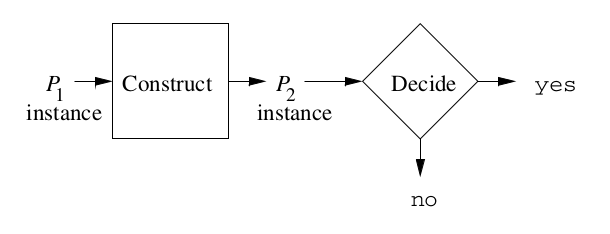
\includegraphics[width=0.5\textwidth]{reduccion.png}
\caption{\label{fig:Reduccion}Esquema de reducción\cite{hopcroft2001introduction}}
\end{figure}
Sin embargo, la existencia de un algoritmo llamado ``Construct'' no es suficiente para probar ``Si $P_1$ no está en $\mathcal{P}$ entonces $P_2$ tampoco está en $\mathcal{P}$''.

Por ejemplo, supongamos que dada una instancia de $P_1$ de longitud $m$ el algoritmo produce una cadena de salida $2^{m}$ la cual entra en nuestro hipótetico algoritmo de tiempo polinomial $P_2$. Si ese algoritmo toma un tiempo polinomial $\mathcal{O}(n^k)$ entonces la salida para una cadena de longitud $2^{m}$ toma un tiempo $\mathcal{O}(2^{km})$, el cual es exponencial en $m$. Por lo tanto el algoritmo de decisión para $P_1$, con una entrada de longitud $m$ toma un tiempo exponencial en $m$. Estos hechos implican que $P_1 \notin \mathcal{P}$ y $P_2 \in \mathcal{P}$

Otra posibilidad es que el algoritmo que construye una instancia de $P_2$ a partir de $P_1$ produzca una instancia que es polinomial en el tamaño de la entrada, sin embargo puede que no podamos alcanzar la conclusión deseada. Por ejemplo, supongamos que la instancia de $P_2$ construida es del mismo tamaño de $m$, como la instancia $P_1$, pero el algoritmo ``Construct'' toma un tiempo exponencial en $m$, como $\mathcal{O}(2^{m})$. Ahora, un algoritmo de decisión para $P_2$ toma un tiempo polinomial $\mathcal{O}(n^{k})$ con una entrada de tamaño $n$ implica que hay un algoritmo de decisión para $P_1$ que toma un tiempo $\mathcal{O}(2^{m} + m^{k})$. Nuevamente obtenemos que $P_1 \notin \mathcal{P}$ y $P_2 \in \mathcal{P}$

La restricción correcta para una traslación de $P_1$ a $P_2$ es que requiere un tiempo polinomial sobre el tamaño de la entrada.

\section{El problema de satisfacibilidad}
%Descripción
El problema de la satisfacibilidad booleana es un problema NP-completo\cite{cook1971complexity}.



\subsection{Codificación del problema}

Las variables se identifican con

\section{Demostración}
Para demostrar que SAT es NP-Completo, primero tenemos que demostrar que es de la clase NP.

\subsection{SAT pertenece a la clase NP}
así es

\subsection{SAT pertenece a la clase NP-Completo}


% Ejemplo de figurita que puede ayudar después
%\begin{figure}
%\centering
%\includegraphics[width=0.5\textwidth]{tesla.jpg}
%\caption{\label{fig:tesla}Esta imagen se añadió en el menú Project.}
%\end{figure}


\bibliographystyle{plain}
\nocite{*}
\bibliography{main}

% Nota
%Para las bibliografías está rotísimo, para que salga todo hay que hacer:
% pdflatex main.tex -f
% bibtex main
% pdflatex main.tex -f
% pdflatex main.tex -f
%
% Dos veces al final

\end{document}
